\documentclass[11pt]{beamer}
\title{SBFSEM-tools tutorial}
\author{Sara Patterson}
\institute{University of Washington}
\usetheme{Goettingen}


\usepackage[utf8]{inputenc}
\usepackage[T1]{fontenc}
\usepackage[english]{babel}
\usepackage{amsmath}
\usepackage{amsfonts}
\usepackage{amssymb}
\usepackage{siunitx}
\usepackage{graphicx}
\usepackage{listings}
\usepackage{hyperref}

\definecolor{codegreen}{rgb}{0,0.6,0}
\definecolor{codegray}{rgb}{0.5,0.5,0.5}
\definecolor{codepurple}{rgb}{0.58,0,0.82}
\definecolor{backcolour}{rgb}{0.95,0.95,0.92}

\lstdefinestyle{mystyle}{
	backgroundcolor=\color{backcolour},   
	commentstyle=\color{codegreen},
	keywordstyle=\color{magenta},
	numberstyle=\tiny\color{codegray},
	stringstyle=\color{codepurple},
	basicstyle=\footnotesize,
	breakatwhitespace=false,         
	breaklines=true,                 
	captionpos=b,                    
	keepspaces=true,                 
	numbers=left,                    
	numbersep=5pt,                  
	showspaces=false,                
	showstringspaces=false,
	showtabs=false,                  
	tabsize=2
}
\lstset{style=mystyle}




\begin{document}
% --------------------------------------------------- Slide --
	\maketitle
% --------------------------------------------------- Slide --
	\begin{frame}
		\tableofcontents
	\end{frame}
% --------------------------------------------------- Slide --
	\section{SBFSEM-tools}
\begin{frame}
	\frametitle{SBFSEM-tools}
	Goal: basic analysis support requiring minimal setup and background in computers, math, etc.
	\vskip10pt
	Current capabilities:
	\begin{itemize}
		\item Import relevant Tulip data (single neurons and networks)
		\item Count up synapses and condense synapses spanning multiple slices 
		\item Summarize synapses with statistics and plots
		\item Sync with Blender images and cell fills
		\item Basic network analysis
	\end{itemize}
	Next:\\
	\begin{itemize}
		\item Compare neurons
		\item Additional network analysis
	\end{itemize}
\end{frame}
% --------------------------------------------------- Slide --
\section{Install}
% --------------------------------------------------- Slide --
\begin{frame}[fragile]
	\frametitle{Install}
	First download or clone \href{www.github.com/sarastokes/sbfsem-tools}{\textcolor{blue}{SBSFEM-tools}}.
	This requires two open-source toolboxes, \href{https://www.mathworks.com/matlabcentral/fileexchange/33381-jsonlab--a-toolbox-to-encode-decode-json-files}{JSONLab} and the \href{https://www.mathworks.com/matlabcentral/fileexchange/47982-gui-layout-toolbox}{\textcolor{blue}{GUI Layout Toolbox}}. I included JSONLab but it will be easier for you to install the GUI Layout Toolbox yourself from Mathworks.\\
	Make sure SBSFEM-tools is added to your MATLAB path like so:
	\begin{lstlisting}[language=matlab]	
	addpath(genpath('C:\...\sbfsem-tools'));\end{lstlisting}
	If you already have JSONLab installed, make sure 
	\begin{lstlisting}[language=matlab] 
	which loadjson\end{lstlisting} 
	returns the version in sbfsem-tools. Otherwise, you might get some errors.
\end{frame}
% --------------------------------------------------- Slide --
\section{Import}
% --------------------------------------------------- Slide --
\subsection{Tulip}
\begin{frame}[fragile]
	\frametitle{Import}
	\framesubtitle{Step One: Tulip}
	\begin{block}{}
		Open a cell in Tulip and then open the Python command line. It's on the bottom toolbar.\\
		Set the file name* and file path:
		\begin{lstlisting}[language=python]
outputFile = "C:\...\c207.json"\end{lstlisting}
		Then run these two lines:
		\begin{lstlisting}[language=python]
params = tlp.getDefaultPluginParameters('JSON Export', graph)
success = tlp.exportGraph('JSON Export', graph, outputFile, params)\end{lstlisting}
	\end{block}
\end{frame}

% --------------------------------------------------- Slide --
\begin{frame}
	\frametitle{Import}
	\framesubtitle{Step One: Tulip}
	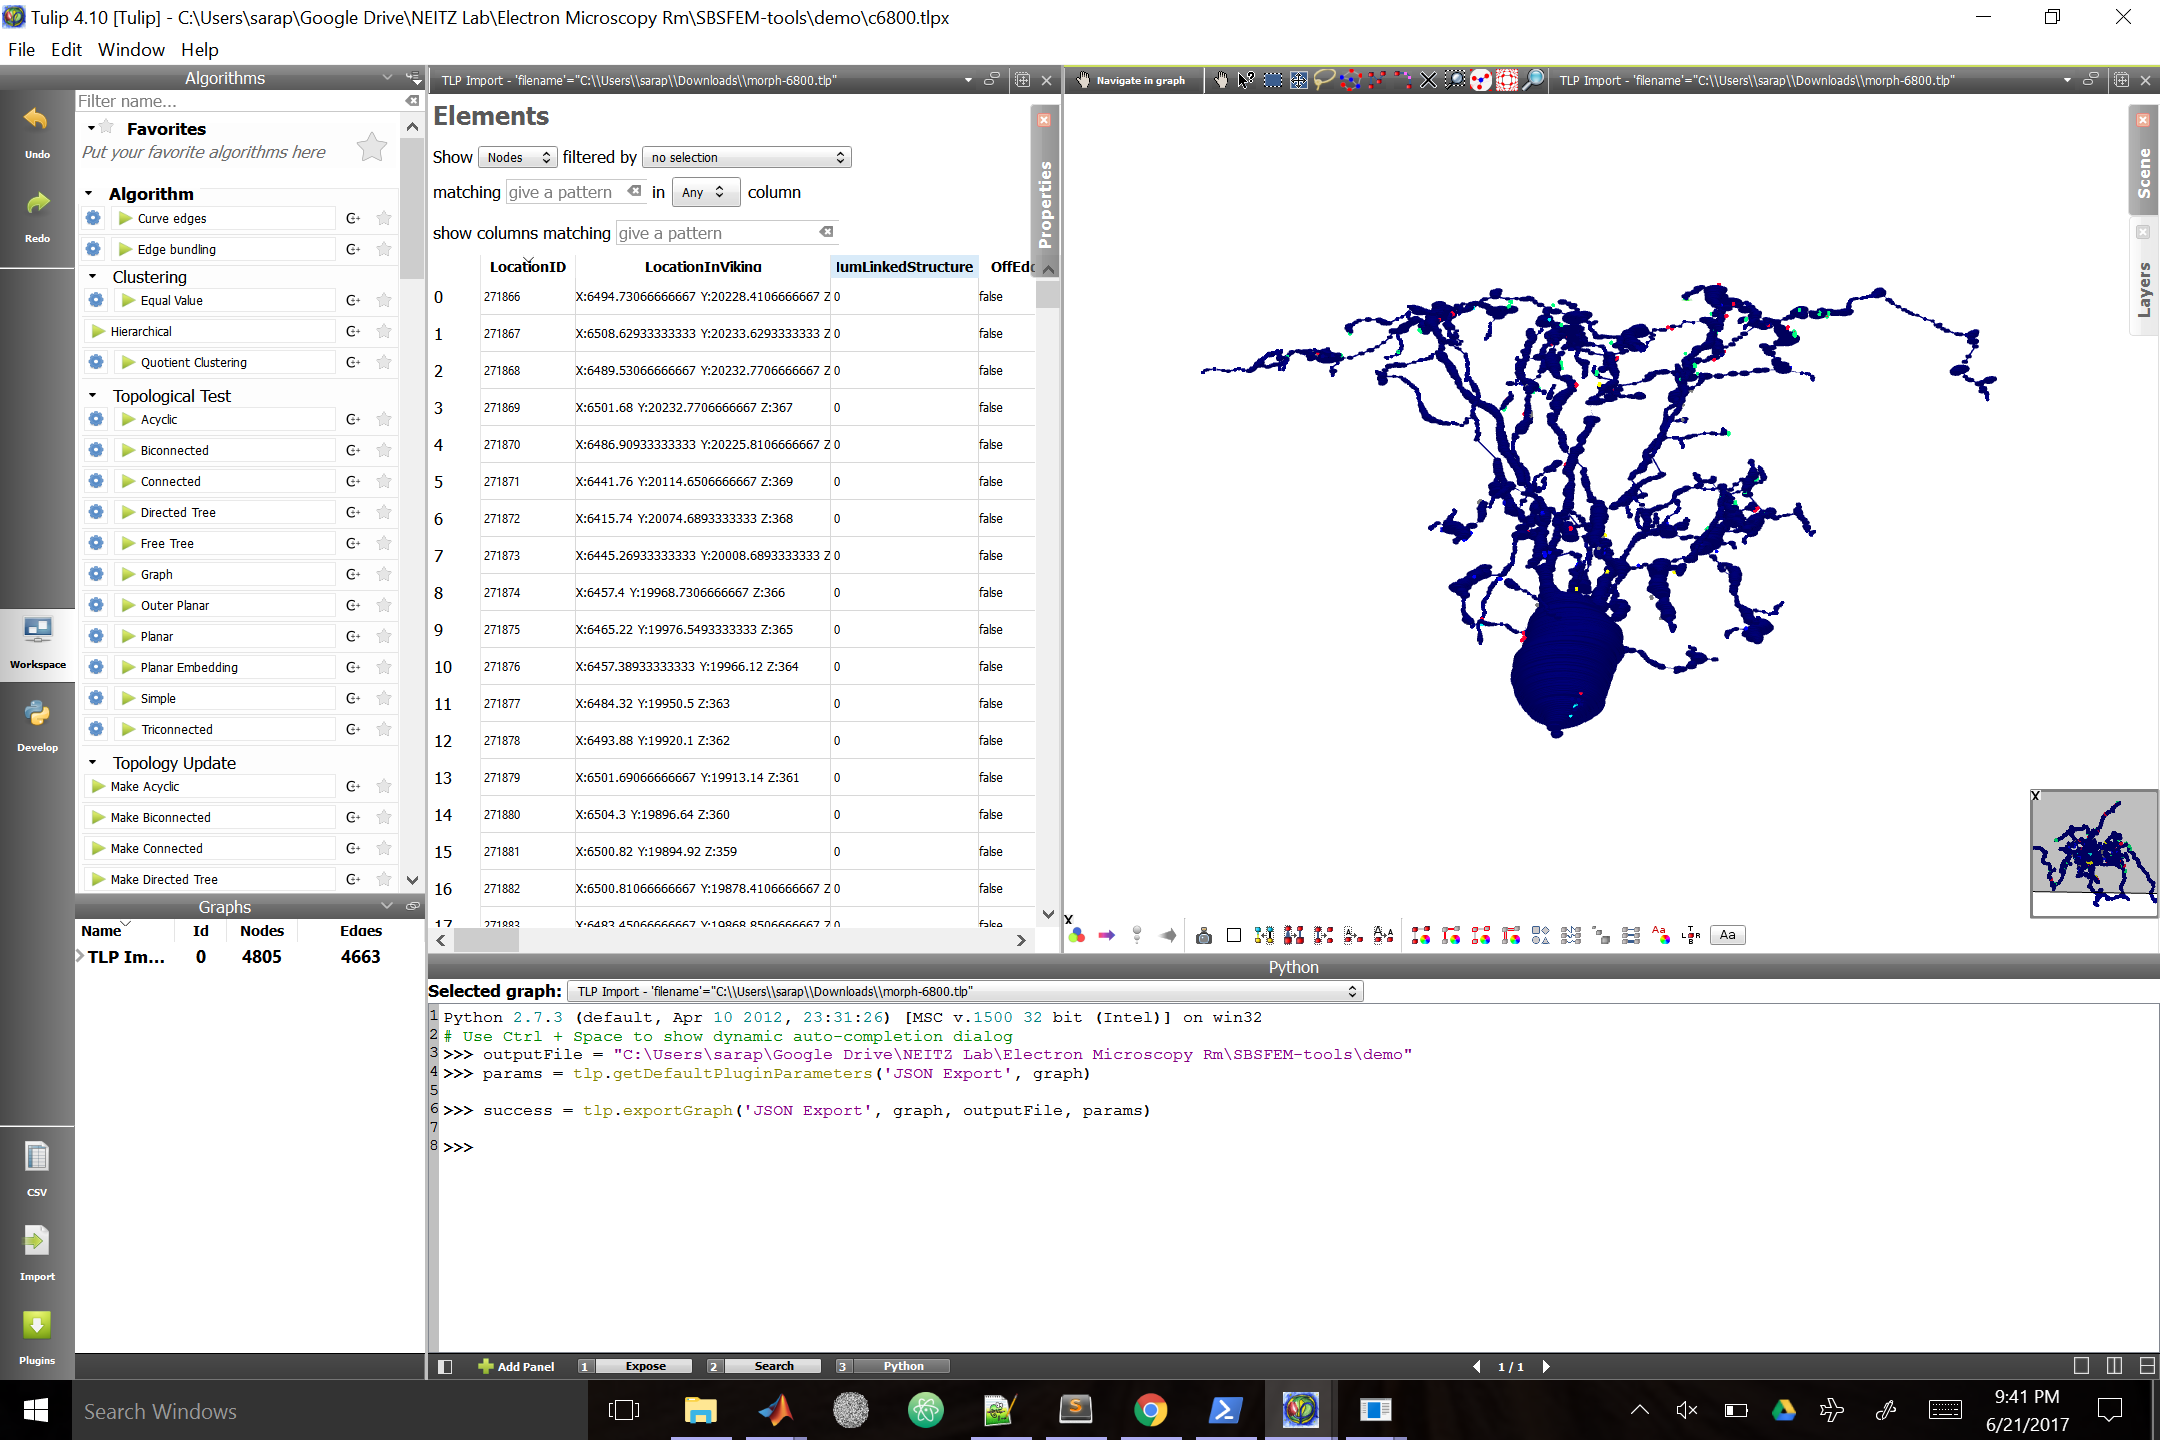
\includegraphics[width = 0.9\textwidth]{tulip_python}
\end{frame}
% --------------------------------------------------- Slide --
\subsection{Matlab}
\begin{frame}[fragile]
	\frametitle{Import}
	\framesubtitle{Step Two - MATLAB}
	Load in the JSON file and create a Neuron object:
	\begin{lstlisting}[language=matlab]
c207 = Neuron('c207.json');\end{lstlisting}
	A dialog box will ask for the cell number. To avoid that, include the cell number while creating the Neuron object:
	\begin{lstlisting}[language=matlab]
c207 = Neuron('c207.json', 207);\end{lstlisting}
	Open up the UI:
	\begin{lstlisting}[language=matlab]
c207.openUI;\end{lstlisting}
\end{frame}
% --------------------------------------------------- Slide --
	\section{User Interface}
	\subsection{Cell Info}
% --------------------------------------------------- Slide --
	\begin{frame}
		\frametitle{Cell Info Panel}
		\begin{itemize}
			\item \textbf{Set the cell number.} This will be used in report generation and file saving. 
			\item If known, the cell type and subtype will be helpful for connectivity analysis.
			\item The other properties will eventually be used for cell queries but don't have much use yet.
		\end{itemize}
			After changing any of the attributes on the Cell Info Panel, make sure to press the \texttt{[Add to cell data]} button. This will make sure your changes are reflected next time you open the UI.\\
	\end{frame}
% --------------------------------------------------- Slide --
	
	\subsection{3d plot}
% --------------------------------------------------- Slide --
\begin{frame}
	\frametitle{3d plot}
	\framesubtitle{Components}
		You can add and remove each synapse type, the soma node and the skeleton independently using the checkboxes.\\Rotate the plot with the elevation and azimuth sliders.
		\vskip20pt
		\begin{columns}
			\column[]{0.5\textwidth}
				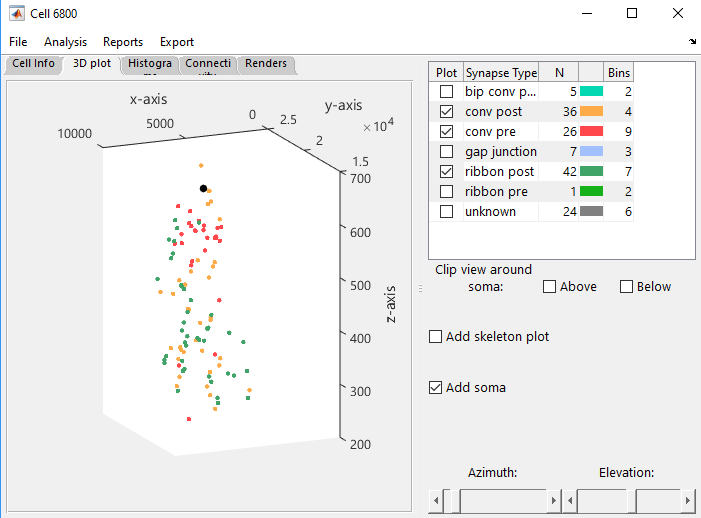
\includegraphics[width=\textwidth]{c6800_plot3}
				\vskip5pt
				AII amacrine cell synapses
			\column[]{0.5\textwidth}
				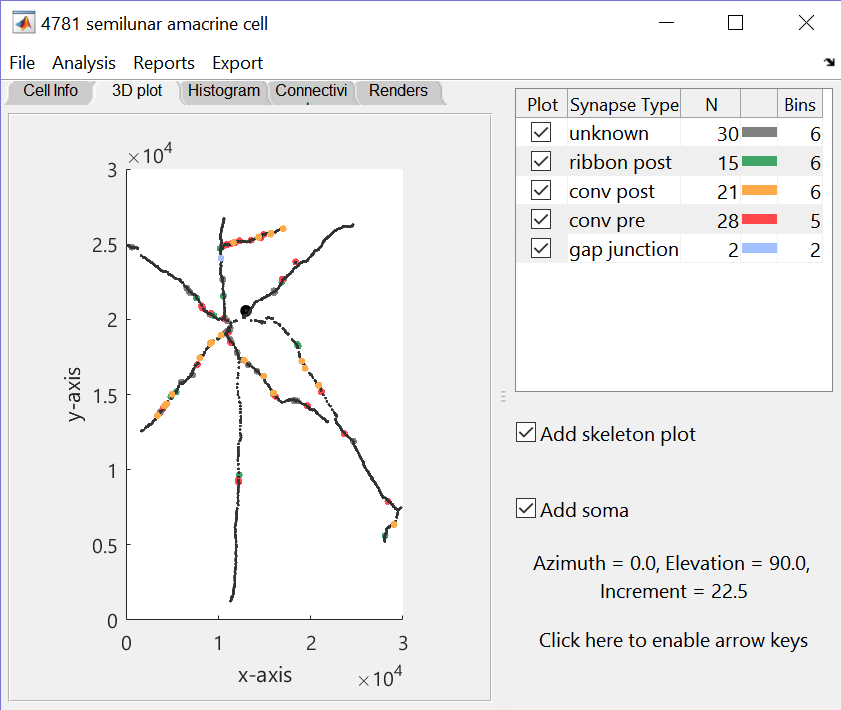
\includegraphics[width=\textwidth]{c4781_plot3}
				\vskip5pt
				Semilunar synapses \& skeleton
		\end{columns}
\end{frame}
% --------------------------------------------------- Slide --	
\subsection{Histograms}
% --------------------------------------------------- Slide --
\begin{frame}
	\frametitle{Histograms}
	\begin{columns}
		\column[]{0.5\textwidth}
			There are two histograms. These plot synapse count as a function of:
			\begin{itemize}
				\item Distance from soma
				\item Section number (z-axis)
			\end{itemize}
		Use the Synapse Table to edit the number of bins.
		\column[]{0.5\textwidth}
			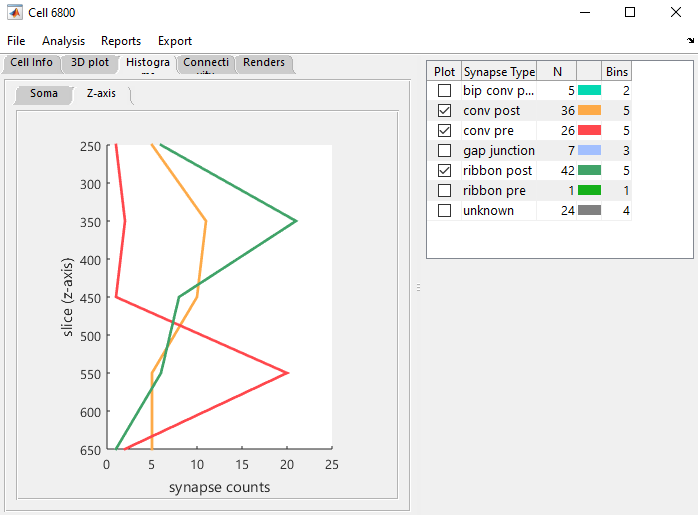
\includegraphics[width=\textwidth]{c6800_histZ}
		\vskip3pt
		Z-axis synapse distribution for a putative AII AC. This synapse asymmetry isn't news but is still good to see.
	\end{columns}
\end{frame}
% --------------------------------------------------- Slide --
\subsection{Connectivity}
\begin{frame}[fragile]
	\frametitle{Connectivity}
	To add connectivity data, save a network map in Tulip as a JSON file, as described above. Then in Matlab:
	\begin{lstlisting}[language=matlab]
c207.addConnectivity('c207hops.json');\end{lstlisting}
	\vskip10pt
	\begin{columns}
		\column[]{0.5\textwidth}
		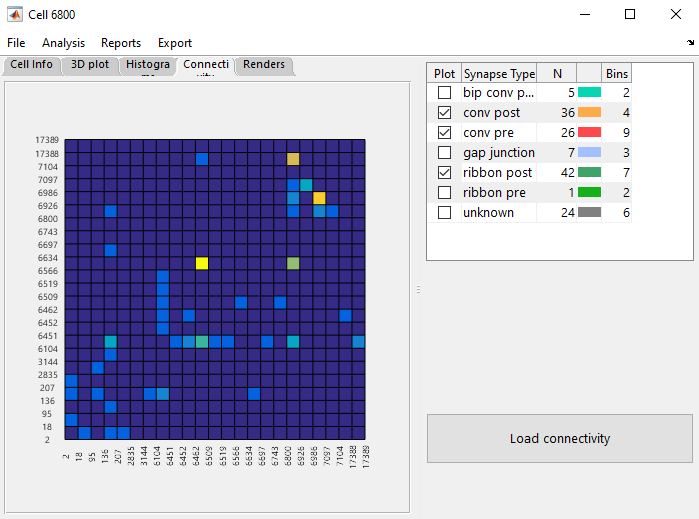
\includegraphics[height=0.4\textheight]{c6800_network}	
		\vskip10pt
		Connectivity for the AII AC.
		\column[]{0.5\textwidth}
		The connectivity matrix is weighted by the number of unique synapses between two cells (dark blue for 0 synapses). Directed synapses will only register a contact from the pre $\rightarrow$ post-synaptic neuron.
	\end{columns}

\end{frame}
% --------------------------------------------------- Slide --
\subsection{Renders}
\begin{frame}
	\frametitle{Blender Renders and Cell Fills}
	\begin{columns}
		\column[]{0.5\textwidth}
		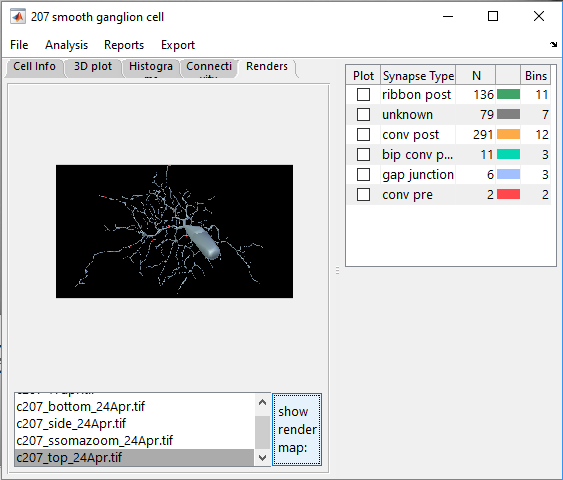
\includegraphics[width=0.9\textwidth]{c207_render}
		\hskip10pt
		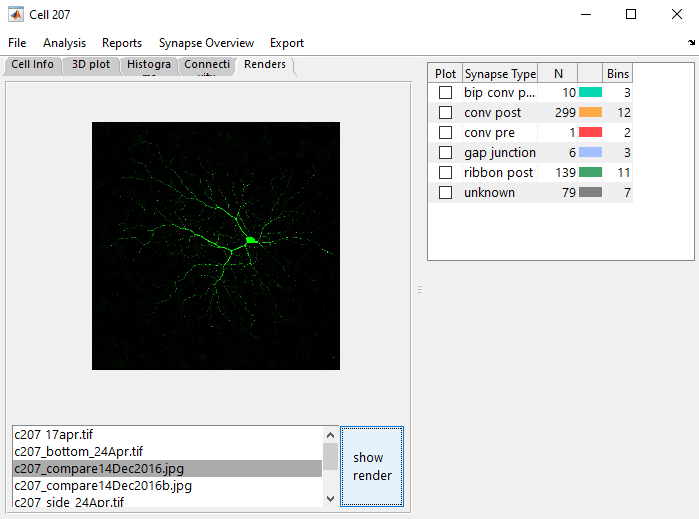
\includegraphics[width=0.9\textwidth]{c207_cellfill}
		\column[]{0.5\textwidth}
		For now, set the \texttt{renderDir} in \texttt{getFilepaths.m} to the file your images are saved into. The UI find the images if their filename includes the letter `c' followed by cell number (like `c207'). I hope to improve this at some point.
		\vskip15pt
		I also include other helpful images. For example, a comparison of the ON-smooth cell I reconstructed to a macular ON-smooth cell I filled.
	\end{columns}
\end{frame}
% --------------------------------------------------- Slide --
\section{Save}
% --------------------------------------------------- Slide --	
	\begin{frame}
		\frametitle{Save}
		\begin{block}{Save Cell Info}
			After adding information to the Cell Info Panel, make sure to press the button \texttt{[Add to cell info]}.\\ This saves cell attributes to the Neuron object.
		\end{block}
		\begin{block}{Save Neuron}
			To save the Neuron object itself, go to \texttt{File-->Save Cell}. Use the UI (not the command line) for saving neurons as this method produces a more compact file size.\\ Note: this is separate from the Cell Info panel save. Also, this will close the UI.  
		\end{block}
	\end{frame}

	\section{Reports}
	\begin{frame}
		\frametitle{Reports}
		This is pretty limited... Right now you can generate two reports:
		\begin{itemize} 
			\item Location IDs of unknown synapses
			\item An overview of all synapse types
		\end{itemize}
		 The report name is auto-generated and will overwrite any existing reports of the same type for that neuron.\\Let me know any other reports that would be of use.
	\end{frame}
% --------------------------------------------------- Slide --
% --------------------------------------------------- Slide --
\section{Organization}
\begin{frame}
	\frametitle{Organization}
	This is boring but will be important for later neuron comparison code...
	\begin{itemize}
		\item Once you pick a folder to save your neuron data in, make a subfolder for each block(for example, \texttt{NeitzTemporal} and \texttt{NeitzInferior}). Save your neurons in these folders. Make a subfolder in each called \texttt{connectivity} and save networks there.
		\item Name the neurons with `c' followed by the cell number - c6800, c207, etc. This will keep the names consistent and make it easier for the program to find data.
	\end{itemize}
\end{frame}
% --------------------------------------------------- Slide --

	\section{Configuration}
% --------------------------------------------------- Slide --	
	\begin{frame}
		\frametitle{Configuration}
			These are found in the \texttt{defaults} folder.
			\begin{enumerate}
				\item \textbf{Directories} - to save time navigating to the correct directory each time, edit \texttt{getFilepaths.m}
				\item \textbf{Cell types and subtypes} - go to \texttt{getCellTypes.m} and \texttt{getCellSubtypes.m}. Let me know if any are missing.
				\item \textbf{Synapse colors} - go to \texttt{getStructureColors.m} to change the default colors for each synapse. 
				%Matlab accepts RGB values between 0-1. Additionally, I included a function to convert hex to RGB \texttt{hex2rgb('0000ff')} and a function to convert color names to RGB (\texttt{rgb('color name')}) - based on \href{https://xkcd.com/color/rgb/}{\textcolor{blue}{XCKD's color survey}}. }
			\end{enumerate}
	\end{frame}

% --------------------------------------------------- Slide --
\begin{frame}
	\frametitle{Links}
	\begin{itemize}
		\item \href{www.github.com/sarastokes/sbfsem-tools}{SBFSEM-tools repository}
		\item \href{https://www.mathworks.com/matlabcentral/fileexchange/47982-gui-layout-toolbox}{GUI Layout Toolbox}
		\item \href{https://www.mathworks.com/matlabcentral/fileexchange/33381-jsonlab--a-toolbox-to-encode-decode-json-files}{JSONLab}
		\item Tulip
		\item Tulip Python documentation
		\item Blender
		\item Viking documentation
	\end{itemize}
\end{frame}	
\end{document}